\chapter{Design}
\label{chap:design}

This chapter is the design of phase 3 (Section~\ref{sec:phases}), the system as built on 23 October 2026. Section~\ref{sec:architecture} gives the architecture and Section~\ref{sec:hardware} the hardware; the software follows (Sections~\ref{sec:dual-imu-architecture} to~\ref{sec:camera-subsystem}), then communications and logging (Section~\ref{sec:mqtt-networking}), the faults that shaped the design (Section~\ref{sec:faults-summary}), the testing tools (Section~\ref{sec:bench-tools}) and maintenance (Section~\ref{sec:maintenance}). Each section names the requirements of Table~\ref{tab:requirements-mapping} and the research questions it serves, and gives what the part does, the key decision and why; pins, formats, parameters and version history are in Appendix~\ref{app:impl}, the firmware configuration in Table~\ref{tab:config} and every connection in Appendix~\ref{app:wiring}. Each interface was tested on its own before higher-level functions were added, so that a fault could be traced to one change.

\section{System overview and architecture selection}
\label{sec:architecture}

This section serves all thirteen requirements, R1 and R7 in particular. Figure~\ref{fig:system-architecture} shows the system. An ESP32-S3 telemetry unit beside the battery, the rear node, samples an inertial measurement unit (IMU), reads GNSS and the battery-management system (BMS), computes ride features, logs locally and publishes over LTE. Since 22 October a second ESP32-S3, the front node, samples a second IMU at the front of the vehicle (Section~\ref{sec:front-node}); until then both IMUs were on the rear unit. Two camera units each run the detector and fuse it with three time-of-flight sensors: the dashboard computer, a Raspberry Pi~5, faces forward and reads the front node over USB; a Raspberry Pi~4 beside the battery faces backward and reads the rear node over a wired UART. An Ethernet cable joins the two (Section~\ref{sec:two-sided}).

\begin{figure}[htbp]
\centering
% System as built, 21 October 2026: two-sided layout (Pi 5 front, Pi 4 rear, Ethernet), ESP32 on a wired UART.
% Sources: TelemetryUnit/src/main.cpp (v0.7.4.1), Server/sw7_ingest.py, CameraDetection/telemetry_bridge.py,
% hazard_detector.py, sensor_fusion.py, sync_logger.py, DashboardIntegration/deploy (pi5-hazard-detector,
% pi5-tof-bridge), live_data_provider.py, sw7_endpoints.py. Dashed amber = not yet working.
\begin{tikzpicture}[x=1cm, y=1cm]
  \def\tw{3.9cm}
  % ---- telemetry unit ----
  \node[swbox, text width=\tw] (a1) at (2.2,-1.5) {%
    2 IMUs, MPU6050, I\textsuperscript{2}C, 200\,Hz each\\
    GNSS receiver in the modem\\
    Battery BMS over Bluetooth LE};
  \node[swplanned, text width=\tw] (a0) at (2.2,-3.0) {Motor Hall tap through an optocoupler (not yet wired)};
  \node[swbox, text width=\tw] (a2) at (2.2,-4.5) {FreeRTOS tasks:\\ ride features, dual-IMU fusion,\\ buffered log in flash};
  \node[swbox, text width=\tw] (a3) at (2.2,-6.2) {LTE modem (A7670X)};
  % ---- Raspberry Pi 4: rear unit ----
  \node[swbox, text width=\tw] (b1) at (7.7,-0.9) {Rear camera, OV5647 NoIR};
  \node[swbox, text width=\tw] (b2) at (7.7,-2.3) {\texttt{hazard\_detector.py}\\ :8080 video, alerts, detections};
  \node[swbox, text width=\tw] (b4) at (7.7,-4.5) {\texttt{telemetry\_bridge.py} with \texttt{sensor\_fusion.py}\\ :8081 telemetry, rear hazards};
  \node[swbox, text width=\tw] (b3) at (7.7,-6.2) {3 ToF sensors, VL53L0X, I\textsuperscript{2}C};
  \node[swbox, text width=\tw] (b5) at (7.7,-7.5) {\texttt{sync\_logger.py}, GPIO17 edges};
  % ---- Raspberry Pi 5: dashboard and front unit ----
  \node[swbox, text width=\tw] (c3) at (13.2,-2.3) {Pages on the 1280\,$\times$\,800 touch screen: driving, Surroundings (front or rear), map};
  \node[swbox, text width=\tw] (c2) at (13.2,-4.5) {\texttt{live\_data\_provider.py}\\ polls every 0.5\,s};
  \node[swbox, text width=\tw] (f1) at (13.2,-6.2) {Front camera, OV5647, and 3 ToF sensors, VL53L0X};
  \node[swbox, text width=\tw] (f2) at (13.2,-7.6) {\texttt{hazard\_detector.py} :8080 and ToF bridge with \texttt{sensor\_fusion.py} :8082};
  \node[swbox, text width=\tw] (c4) at (13.2,-9.3) {\texttt{sw7\_ingest.py}: SQLite database, one copy per record};
  % ---- outside the vehicle ----
  \node[swbox, draw=swGrey, fill=white, text width=\tw] (mq) at (2.2,-9.3) {Public MQTT test broker};
  \node[swbox, draw=swGrey, fill=white, text width=\tw] (net) at (13.2,-0.6) {Internet: OpenStreetMap tiles, OSRM routes};

  % ---- lanes (drawn behind) ----
  \begin{scope}[on background layer]
    \node[swlane, fit=(a1)(a0)(a2)(a3), minimum width=4.6cm] (la) {};
    \node[swlane, fit=(b1)(b2)(b4)(b3)(b5), minimum width=4.6cm] (lb) {};
    \node[swlane, fit=(c3)(c2)(f1)(f2)(c4), minimum width=4.6cm] (lc) {};
  \end{scope}
  \node[swlanetitle] at (la.north west) {Telemetry unit (ESP32-S3, v0.7.4.1)};
  \node[swlanetitle] at (lb.north west) {Raspberry Pi~4: rear, by the battery};
  \node[swlanetitle] at (lc.north west) {Raspberry Pi~5: front};

  % ---- links inside each unit ----
  \draw[swflow] (a1) -- (a0);
  \draw[swflow] (a0) -- (a2);
  \draw[swflow] (a2) -- (a3);
  \draw[swflow] (b1) -- (b2);
  \draw[swflow] (b2) -- node[swlabel, right=1pt] {detections, 5\,Hz} (b4);
  \draw[swflow] (b3) -- (b4);
  \draw[swflow] (c2) -- node[swlabel, right=1pt] {live state} (c3);
  \draw[swflow] (f1) -- (f2);
  \draw[swflow] (f2.east) -- ++(0.25,0) |- node[swlabel, pos=0.25, right=1pt, align=left] {front video,\\ alerts, ToF} (c2.east);
  \draw[swflow] ($(net.south)+(1.3,0)$) -- ($(c3.north)+(1.3,0)$);

  % ---- links between units ----
  \draw[swlink] (a2.east) -- node[swlabel, above=2pt] {UART,\\ 460\,800\,Bd,\\ \texttt{DASH} 1\,Hz} (b4.west);
  \draw[swlink] ($(a2.east)+(0,-0.4)$) -- (4.95,-4.9) -- (4.95,-7.5) -- (b5.west);
  \node[swlabel, rotate=90, anchor=south] at (4.95,-6.3) {sync pulse, 500\,ms};
  \draw[swlink] ($(b4.east)+(0,0.15)$) -- node[swlabel, above=2pt] {Ethernet,\\ HTTP} ($(c2.west)+(0,0.15)$);
  \draw[swlink] (b2.east) -- node[swlabel, above=2pt] {rear video,\\ alerts} (c3.west);
  \draw[swlink] (a3) -- node[swlabel, left=1pt] {MQTT over LTE,\\ every 10\,s, replays} (mq);
  \draw[swlink] (mq.east) -- node[swlabel, above=2pt] {MQTT subscription over the Internet} (c4.west);
\end{tikzpicture}

\caption{The system as built on 23 October 2026: the Raspberry Pi~5 beside the display runs the dashboard, the front camera unit and the front node (a second ESP32-S3 with one IMU, Section~\ref{sec:front-node}); the Raspberry Pi~4 beside the battery runs the rear camera unit and reads the telemetry unit, now with one IMU; the two are joined by an Ethernet cable (Section~\ref{sec:two-sided}). A phone's GNSS gives speed (Section~\ref{sec:impl-phone-gps}). Programs are named by their files in the repository. Dashed outline: built but not yet connected on the vehicle.}
\label{fig:system-architecture}
\end{figure}

Table~\ref{tab:architectures} compares the feasible architectures. The deciding requirements were R1 (a fixed 200\,Hz period with no loss) and R7 (detection at a useful frame rate). A microcontroller under FreeRTOS holds a fixed period but cannot run a camera network at a useful rate; a Raspberry Pi can run the network, but a general-purpose Linux scheduler gives no guarantee of a 5\,ms period. Splitting the work keeps each part where it is predictable. The first camera went on a Raspberry Pi~4 rather than the Raspberry Pi~5 because the Pi~5 runs the inherited dashboard, and developing on it would have put a working deployment at risk. Power was not measured for any option; the one power finding is that the modem must not be powered from a Raspberry Pi's USB port (Section~\ref{sec:full-system-integration}).

\begin{table}[htbp]
\centering
\small
\caption{Feasible architectures compared. Figures are measured in this project unless marked; power was not measured.}
\label{tab:architectures}
\begin{tabular}{|p{2.0cm}|p{2.9cm}|p{1.8cm}|p{1.9cm}|p{2.2cm}|p{2.2cm}|}
\hline
\textbf{Option} & \textbf{Workload} & \textbf{Power} & \textbf{Memory} & \textbf{Interfaces} & \textbf{Latency, timing} \\ \hline
ESP32-S3 alone & Dual 200\,Hz sampling, features, BLE, modem: yes. Camera network at a useful rate: no & Lowest of the options (not measured) & 16\,MB flash, 8\,MB PSRAM (not used) & Two I\textsuperscript{2}C, UARTs, BLE, native USB; LTE and GNSS on the board & 5\,ms period held, 200.0 to 200.5\,Hz \\ \hline
Raspberry Pi alone & Detector at 19.5\,frames/s (Pi~4); fixed-period sampling not guaranteed & Higher; under-voltage on a weak supply & Not a constraint in testing & I\textsuperscript{2}C, CSI camera, Wi-Fi, USB; no LTE modem & Detector 102\,ms median; sampling jitter not bounded by design \\ \hline
ESP32-S3 and Pi~4 (chosen) & Acquisition on the ESP32, vision and fusion on the Pi & Two supplies; modem not from the Pi's USB & As above & Pulse wire for timing; wired UART for data (USB until 21 October) & 5\,ms acquisition; 102\,ms detection alone, 118 to 122\,ms with the whole system; 1\,Hz dashboard line \\ \hline
Pi~5 with Hailo-8 accelerator (not tested) & Detector at camera rate expected; no Pi~4 link needed & Not measured & 16\,GB & Accelerator not yet enabled on the PCIe bus & Not measured \\ \hline
\end{tabular}
\end{table}

\section{Hardware}
\label{sec:hardware}
\label{sec:camera-mount}

This section serves R1, R4, R5, R6, R8 and R13. The telemetry unit is a Makerfabs ESP32-S3 board with an A7670X LTE Cat-1 modem that also contains the GNSS receiver \cite{makerfabsa7670x} (Figure~\ref{fig:makerfabs-pinout}, Appendix~\ref{app:figures}); the integrated board let processor, modem and GNSS be tested without a separate modem circuit. Each IMU (MPU6050) has its own I\textsuperscript{2}C bus, which avoids their shared address and bus contention. Each camera unit carries an OV5647 camera without an infrared-cut filter and three VL53L0X time-of-flight sensors, in a casing designed and printed in this project (Figure~\ref{fig:camera-casing}). The enclosures and mounts that put the system on the vehicle, and the checks on their geometry, are in Appendix~\ref{app:mechanical}; the pins, the bench setup (Figure~\ref{fig:bench-setup}) and why the board's microSD slot was not used are in Section~\ref{sec:impl-hardware}.

\section{Firmware architecture}
\label{sec:dual-imu-architecture}
\label{sec:acquisition-instrumentation}

This section serves R1 and R6, and RQ1 and RQ3. The firmware (PlatformIO, Arduino on FreeRTOS) builds both nodes from one source. Each IMU task runs at the highest priority on core~1 and holds a 5\,ms period with \texttt{vTaskDelayUntil}, which schedules each wake-up from the previous target so that execution time does not accumulate into drift; the modem, BMS and dashboard-line tasks, and since v0.7.6 the statistics and ride tasks, run on core~0, so that processing never shares a core with acquisition (Section~\ref{sec:inv-stall}). The 200\,Hz rate exceeds the 160\,Hz Nyquist rate of the 80\,Hz upper limit of the ISO~2631-1 band \cite{iso2631}, with margin. Each sample carries a sensor identifier, a sequence number and a microsecond timestamp; no acquisition task prints, and a full queue drops and counts the new sample rather than block, so a slow consumer can never hold up sampling. A statistics task reports each sensor's rate, interval range and drops every 2\,s, so the acquisition results need no separate measurement pass. The IMUs run at $\pm 8\,g$ and $\pm 500^{\circ}$/s with a 94\,Hz low-pass filter (from v0.7.4), the widest below the 100\,Hz Nyquist frequency. The task diagram (Figure~\ref{fig:task-architecture}), catch-up and late-slot rules are in Section~\ref{sec:impl-fw}.

\subsection{Raw sample stream}
\label{sec:raw-stream}

Up to v0.7.4.1 only the 1\,s features left the unit, so the first road session kept no samples. Since v0.7.5 every sample goes to the Raspberry Pi as hex text lines, each ending in a CRC-16, on the same link as the dashboard line, through a lowest-priority sender that gives a line up rather than delay the dashboard line. Text was chosen over binary to keep the stream line-based and readable in a terminal; at about a third of the rear link's capacity the cost is affordable. Sequence numbers count 5\,ms slots, so missing numbers equal read failures plus dropped lines. The line formats are in Section~\ref{sec:impl-raw}.

\subsection{Sensor health and recovery}
\label{sec:imu-health}

Since v0.7.5 each read is classed as good, failed or stuck, and v0.7.6 adds consumer ages, highest queue fill, late slots and per-core idle counts to the dashboard line, which together say where a stall is. An MPU6050 that loses power returns asleep and repeats one reading; v0.7.7 re-initialises it after 1\,s of failed or identical reads, without a reset, and v0.7.8 runs local commands at once instead of after the modem's timeouts. Both nodes run v0.7.8 since 22 October, and on that day the recovery was confirmed on the bench: four pulls of IMU1's supply wire, each followed by re-initialisation with no drops and no reset (Section~\ref{sec:impl-health}).

\subsection{Front node}
\label{sec:front-node}

On 22 October the second IMU was moved to its own node at the front, so that the two sensors measure at the two ends of the vehicle (RQ1, RQ4). The front node is a bare ESP32-S3 board built from the same source with one IMU and no modem, BLE or GNSS, powered and read through the Raspberry Pi~5's USB port, with its own sync pulse to that Pi. The two Pis share a time base over the Ethernet cable (Section~\ref{sec:data-collection}). The move also removed IMU2's long wires from the rear unit (Section~\ref{sec:impl-front}).

\section{Ride-characterisation signal processing}
\label{sec:ride-characterisation}

This section serves R2 and R3, and RQ1 and RQ4. A task per IMU computes time-domain features from each one-second window of $N = 200$ samples ($\Delta t = 1/f_s$). The acceleration magnitude is used rather than one axis because the mounting has not been related to a vehicle frame; it does not depend on orientation, at the cost of not saying which axis a disturbance came from. The calibrated magnitude of sample $k$ is
\begin{equation}
a_k = s\,\sqrt{a_{x,k}^2 + a_{y,k}^2 + a_{z,k}^2},
\label{eq:magnitude}
\end{equation}
where $s$ is the sensor's calibration factor. From the window,
\begin{align}
\mu &= \frac{1}{N}\sum_{k=1}^{N} a_k, &
a_{\mathrm{RMS}} &= \sqrt{\frac{1}{N}\sum_{k=1}^{N} a_k^2}, &
\sigma &= \sqrt{\frac{1}{N}\sum_{k=1}^{N} a_k^2 - \mu^2}, \label{eq:mean-rms-std}\\
a_{\mathrm{pp}} &= \max_k a_k - \min_k a_k, &
\mathrm{CF} &= \frac{\max_k a_k}{a_{\mathrm{RMS}}}, &
\bar{J} &= \frac{1}{N-1}\sum_{k=2}^{N} \frac{\lvert a_k - a_{k-1}\rvert}{\Delta t}, \label{eq:pp-cf-jerk}
\end{align}
and the threshold count is the number of samples with $a_k > \mu + 2\sigma$. Because $a_k$ includes gravity, $a_{\mathrm{RMS}}$ is close to 9.8\,m/s\textsuperscript{2} at rest and the crest factor close to 1; $\sigma$ removes the constant part and is the vibration measure used. The ISO~2631-1 frequency weighting is not applied on the unit, so these features describe vibration exposure, not comfort as the standard defines it; the offline analysis of the raw stream computes the weighted value (Section~\ref{sec:road-analysis}). The feature code is checked at every boot against a synthetic sine (Section~\ref{sec:impl-ride}).

\subsection{Per-sensor calibration}
\label{sec:imu-magnitude-calibration}

Two nominally identical sensors at rest read about 8\,\% apart. Since only the magnitude is used, one scale factor per sensor (Equation~\ref{eq:calibration}), measured from 200 stationary readings at first boot and kept in non-volatile storage, corrects it; it is reused rather than recomputed at boot, since the vehicle may be powered while moving, and a console command (\texttt{!recal}) recalibrates in place. A single factor holds only in the orientation in which it was measured, because per-axis offsets remain (Section~\ref{sec:impl-cal}).

\subsection{Speed-normalised index}
\label{sec:speed-norm}

The same road driven faster gives a larger response. Following Li et al., who classify roughness from acceleration mean square divided by speed \cite{li2018}, each window also computes
\begin{equation}
I_v = \frac{\sigma^2}{v}, \qquad v \ge v_{\min},
\label{eq:speed-index}
\end{equation}
where $v$ is the GNSS speed. The GNSS speed has not been checked against a known speed and the sensors are on the body, not the unsprung mass, so $I_v$ supports relative comparison within one dataset, not a roughness class (Section~\ref{sec:impl-speed}).

\subsection{Two-sensor fusion and comparison}
\label{sec:imu-fusion}

While both IMUs were on the rear unit (to v0.7.6, and on the first road session) they measured one motion and were averaged with equal weights, with a disagreement figure $D$ (Equation~\ref{eq:disagreement}) and a fallback to one sensor. Since 22 October the sensors are at the two ends of the vehicle, where a road feature reaches them at different times, so they are reported separately and compared, not averaged: the analysis on the Raspberry Pis gives per-sensor features over common windows and the front-to-rear delay, from which speed follows as the wheelbase divided by the delay (Sections~\ref{sec:road-analysis} and~\ref{sec:impl-fusion}).

\section{Battery-management interface}
\label{sec:bms-interface}

This section serves R5 and RQ3. The pack reports voltage, current, state of charge, temperatures and faults over Bluetooth Low Energy in the JBD protocol. The inherited implementation leaked a client on every reconnection, reconnected on a timer and framed messages by a byte that can occur in the data; it was rewritten with one reused client, reconnection on disconnect, length-based framing, a checksum and a plausibility check, and the field offsets were confirmed against a teammate's independent parser. The link was intermittent until the unit was moved near the pack (Section~\ref{sec:two-sided}). The pack supplied up to 46.9\,A on the road, so it is the traction pack, not the auxiliary pack that inherited documentation suggested (Section~\ref{sec:impl-bms}).

\section{Positioning}
\label{sec:gnss-parsing-validation}
\label{sec:gnss-outdoor}

This section serves R4, and RQ1 and RQ3. The modem's GNSS is polled every 3\,s. Because the available manual \cite{simcoma76xx} was not known to match the fitted modem, the parser was written defensively and logs the raw reply; the real reply did differ (Section~\ref{sec:inv-gnss}), and since v0.5.3 the parser anchors on the latitude hemisphere letter, which fits every observed layout, and rejects a fix with an invalid format or an implausible jump. Assisted GNSS and the modem's network position (about 550\,m accuracy, never used for speed or the ride index) were added in v0.7.3 (Section~\ref{sec:impl-gnss}).

\section{Other vehicle inputs}
\label{sec:environmental-sensing}
\label{sec:hall-tap}

These serve RQ1 and RQ4; no requirement depends on them yet. A Sensirion SEN55 air-quality sensor \cite{sensirionsen5x} was chosen so that conditions along a route share the vehicle's timeline; it is not yet connected. Motor speed would help separate powertrain vibration: firmware v0.6.0 counts the Hall signal, to be tapped through an optocoupler, in the hardware pulse counter at no cost to the IMU tasks, and was checked against the sync pulse as a loopback. The details and open questions are in Section~\ref{sec:impl-other}.

\section{Camera subsystem}
\label{sec:camera-subsystem}

This section serves R6, R7, R8, R10 and R11, and RQ1, RQ2 and RQ3.

\subsection{Capture and synchronisation}
\label{sec:sync-pulse}

The camera's first purpose is a visual record against which inertial events can be labelled. The camera and the IMUs are on different boards, so their clocks are related by a shared signal: the ESP32 toggles a pin every 500\,ms and logs each edge's time, and the Raspberry Pi logs each edge's arrival from the kernel's GPIO character device, on the same monotonic clock as the camera's frame timestamps \cite{picamera2manual}, so frames and edges share one time base. The first logger, a Python callback, had a wider spread and one unexplained gap, which is why the kernel time is used (Section~\ref{sec:impl-sync}).

\subsection{Detection}
\label{sec:hazard-detection}

The detector runs a pretrained SSD-MobileNet-v1 \cite{liu2016ssd, howard2017mobilenets}, trained on COCO \cite{lin2014coco} and quantised to 8-bit integers \cite{jacob2018quantization} for LiteRT \cite{litert}, which needs no training data and no accelerator (Section~\ref{sec:lit-detection}). It reports vehicles, cyclists, pedestrians and animals in three distance bands estimated from box width; the focal length is not yet calibrated, so the bands are indicative. An alert needs three consecutive frames and clears only after five without the object, a rule that came from 16 activations in 47\,s for one person when one missed frame cleared an alert. Data handling is minimal by design and was fixed in code before the first live frame: each alert keeps five fields (class, band, confidence, time, status), frames exist only in memory, there is no recognition of faces or plates, inference is local, and the output is advisory. Per-frame latency is measured from the sensor timestamp. A YOLO11n pothole model \cite{ultralytics2024yolo11} fine-tuned on public and South African data \cite{gerapothole, nienaber2015dataset} runs only as an experimental path, off by default, because it slows the detector \cite{ncnn}. Details are in Section~\ref{sec:impl-detect}.

\subsection{Range sensing and fusion}
\label{sec:tof-sensor}
\label{sec:camera-tof-fusion}

A VL53L5CX (8$\times$8 zones) was chosen for proximity sensing, but had not arrived, so three VL53L0X sensors facing left, ahead and right stand in on each camera unit, on the Pi's own bus so that the ESP32's acquisition is undisturbed. A sensor that does not answer is skipped and looked for again (Section~\ref{sec:inv-tof}). The camera says what an object is and where, but not how far; a time-of-flight sensor measures distance well, but only close by and without a class. A fusion step combines them: a detection whose bearing falls in a sensor's cone, with a fresh valid reading, takes the camera's class and the sensor's distance; an unmatched detection keeps the camera estimate, and a sensor reading with no detection becomes an unclassified obstacle. There is no tracking, and the sensor directions are defaults, not measurements. The gates, geometry (Figure~\ref{fig:fusion-geometry}) and validation plan are in Section~\ref{sec:impl-tof}.

\subsection{Dashboard integration}
\label{sec:dashboard-page}
\label{sec:dashboard-link}
\label{sec:live-only}
\label{sec:pi5-default}

An inspection of the inherited PySide6 dashboard on 2 October found no live input: every page ran on simulated data. A driver's display should not depend on coverage or a remote broker, so a local path was built: the telemetry unit prints one JSON line a second (the dashboard line), a bridge on each Raspberry Pi serves it with the distances and fused hazards over HTTP, and a live-data provider in the dashboard polls it. The design answers the display issues of Section~\ref{sec:lit-display}. Data validity: in live-only mode a field with no live source stays empty and lost data is shown as absent, never replaced by simulation, after the dashboard was seen showing a simulated 82\,\% battery level. Layout: few added elements (a camera page, a Sensors page, a ride-quality card, a front-obstacle distance from the forward sensor only). Colour: the dashboard's own status colours. Priority: only an immediate hazard, or loss of the rear link, raises a banner over every page. The integration is a patch set applied to a separate copy by a script that refuses to touch the team's code, so one command restores the team's dashboard. The details, including discovery of the Raspberry Pi~4 and the map, are in Section~\ref{sec:impl-dash}, and the page redesign in Appendix~\ref{app:interface}.

\subsection{Approaching objects: time to contact}
\label{sec:ttc}

A distance band says how near an object is, not whether it is coming closer. Since 15 October a tracker follows each detection across frames, and the time to contact is estimated from the growth of its image width, $\tau = w/\dot{w}$, the expansion measure of Section~\ref{sec:lit-detection} \cite{lee1976tau,dagan2004fcw}, fitted robustly \cite{sen1968} over the last 0.6\,s; it needs no focal length or object size, which are uncalibrated. An object is ``approaching'' below 4\,s (warning) or 2\,s (immediate). At close range the time-of-flight sensors give their own closing time. The vehicle's own motion makes a stationary object ahead approach, which is intended: it is then a forward-collision warning. The acceptance rules are in Section~\ref{sec:impl-ttc}; the accuracy test (C11) has not been run.

\subsection{Two-sided layout}
\label{sec:two-sided}

On 15 October the hardware was rearranged after two findings: the BMS link did not reach the telemetry unit at the front of the vehicle, and the Raspberry Pi~5 ran the detector with half the Raspberry Pi~4's latency (Section~\ref{sec:res-hazard}). The Raspberry Pi~5 behind the dashboard now runs the front camera, detector and time-of-flight board, so a front alert no longer crosses the network; the Raspberry Pi~4 beside the battery looks backwards and keeps the telemetry unit, near enough for the BMS link. A dedicated Ethernet cable joins them, so Wi-Fi keeps the route to the internet. The dashboard's Surroundings page switches between Front and Rear, the rear view mirrored like a reversing camera, and the banner shows warnings from both sides (Figure~\ref{fig:two-sided}; Section~\ref{sec:impl-twosided}).

\begin{figure}[htbp]
\centering
\subfigure[Surroundings, Front: the Raspberry Pi~5's camera and time-of-flight board (test image).]{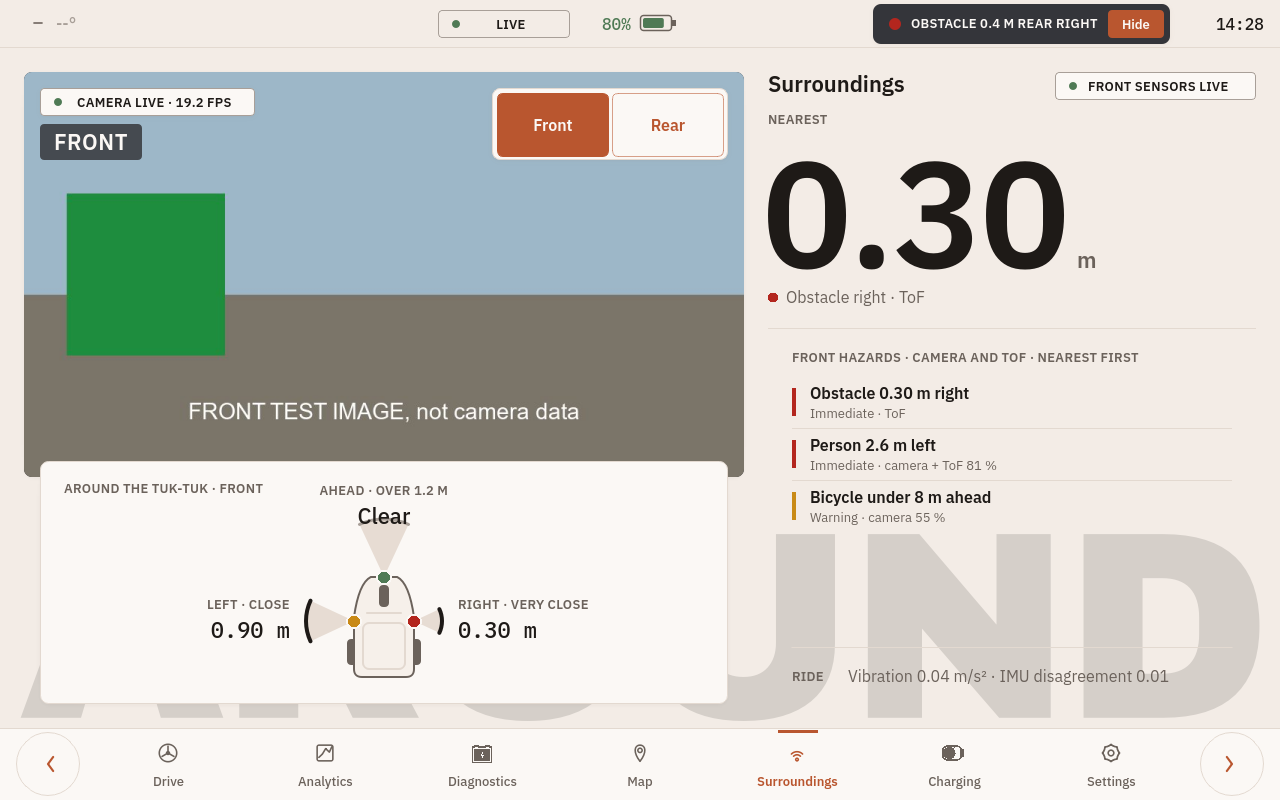
\includegraphics[width=0.48\textwidth]{figures/ui/ui_dualcam_front.png}}
\subfigure[Surroundings, Rear: mirrored, with a car approaching at 1.6\,s (test data).]{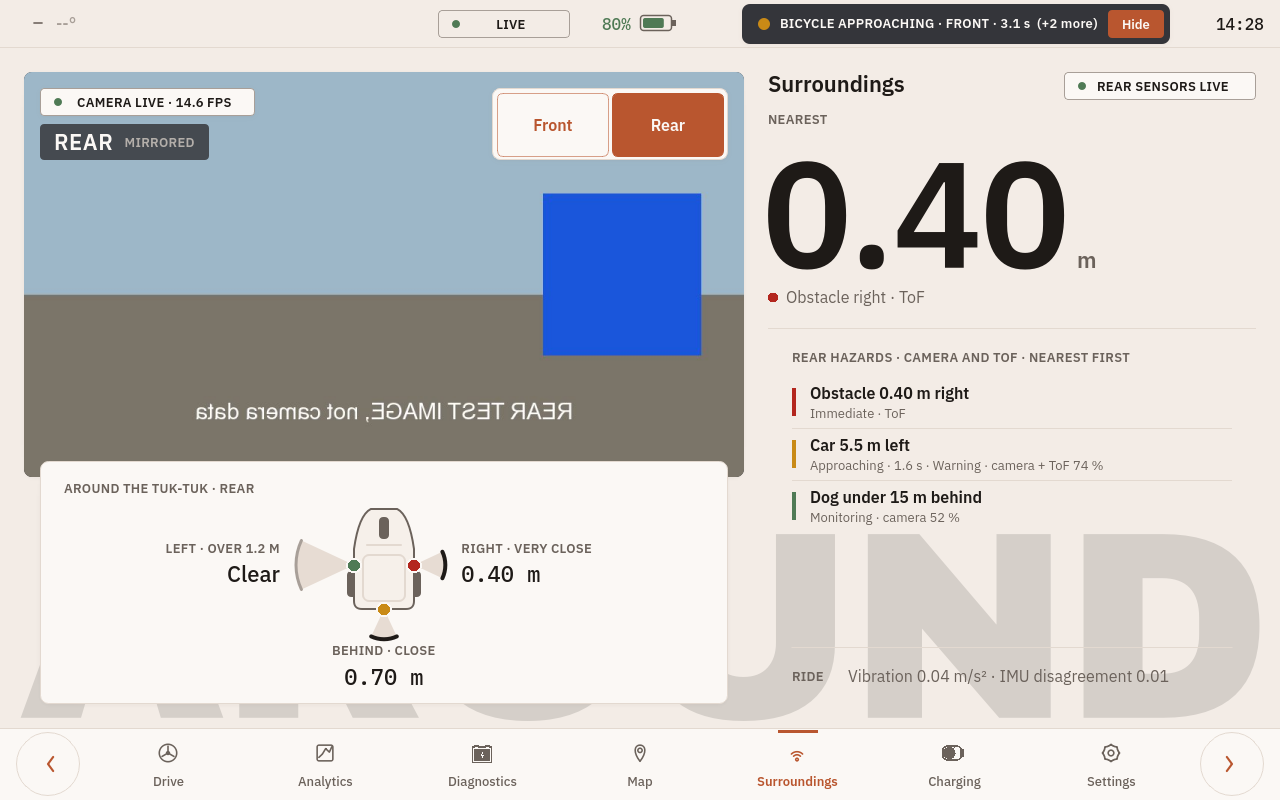
\includegraphics[width=0.48\textwidth]{figures/ui/ui_dualcam_rear_approaching.png}}
\subfigure[On the Raspberry Pi~5 on 15 October: live front camera at 23.6\,frames/s, a rear warning in the banner.]{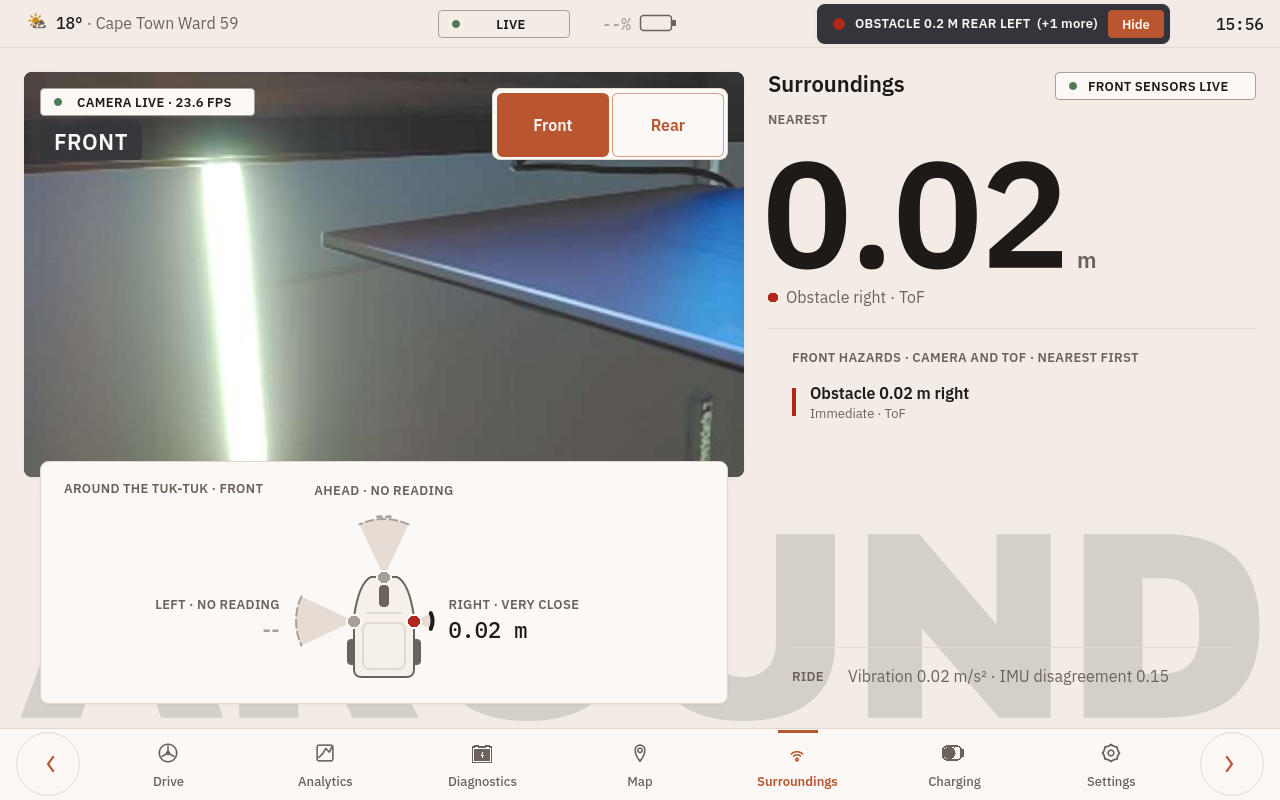
\includegraphics[width=0.48\textwidth]{figures/ui/ui_pi5_live_dualcam.png}}
\subfigure[Front time-of-flight board on the Raspberry Pi~5: the same pins as on the Raspberry Pi~4.]{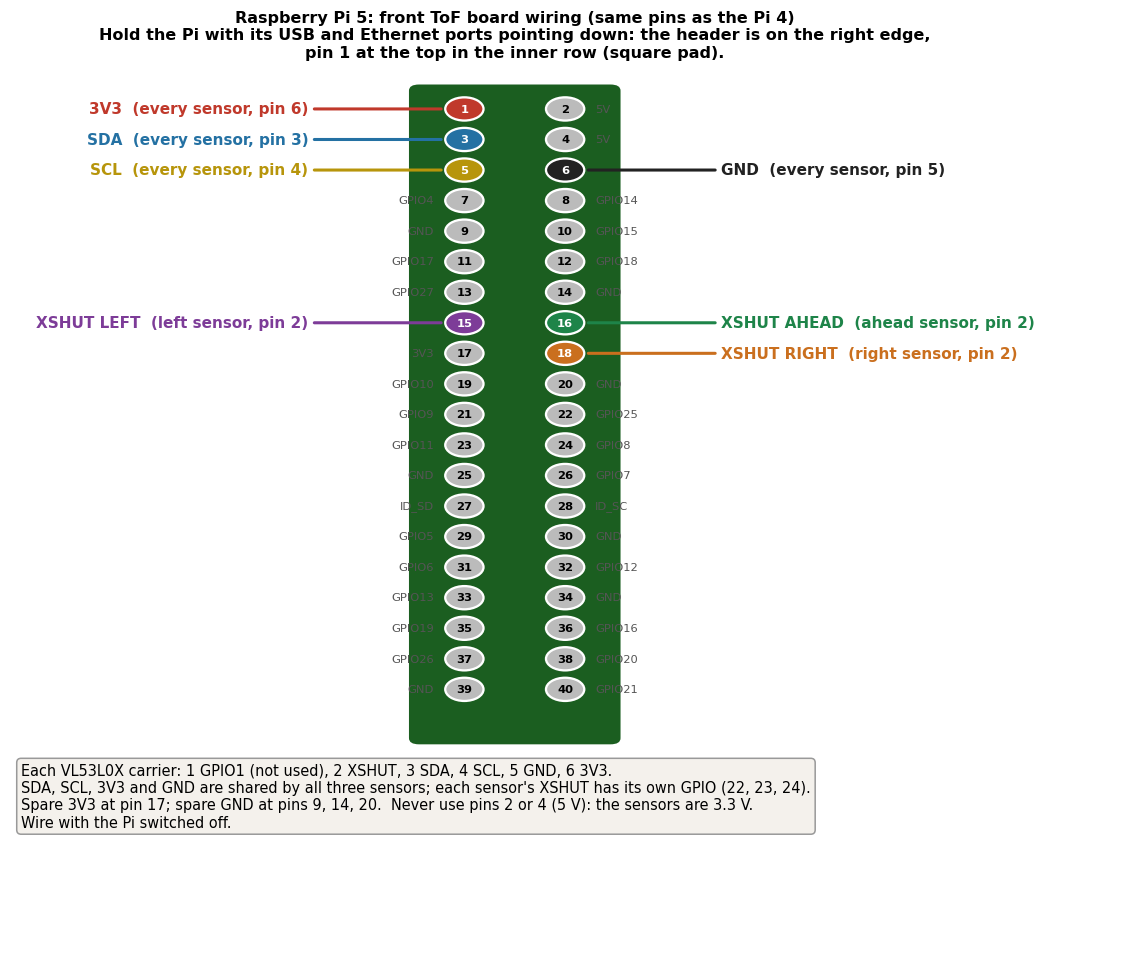
\includegraphics[width=0.48\textwidth]{figures/pi5_tof_wiring.png}}
\caption{Two-sided layout: front sensing on the Raspberry Pi~5, rear sensing and the telemetry unit on the Raspberry Pi~4.}
\label{fig:two-sided}
\end{figure}

\section{Communications and local logging}
\label{sec:mqtt-networking}

This section serves R9 and R10, and RQ3. Every 10\,s the modem task publishes a JSON summary over MQTT using the modem's own commands; publishing stays in that task because the modem UART has no lock. The broker is a public test broker, used only to prove the path, so since v0.7.5 the published record carries no position. The firmware waits for the modem's separate result code rather than trusting its first \texttt{OK}, treats a session as lost on repeated failures or the modem's report, and reconnects as soon as packet data returns.

\label{sec:local-logging}
Every record is also written to flash whatever the coverage, so that a session leaves a complete record. Because flash writes pause code on both cores, records are buffered and written about once a minute (v0.6.0), which makes the pause rarer, not shorter; missing values are written as \texttt{null} so that the log stays valid JSON (Section~\ref{sec:inv-json}).

\label{sec:db-sync}
Store-and-forward (v0.7.4). Every record carries a boot counter and a sequence number that never repeats, and is published with acknowledgement (QoS~1). A ledger tracks the acknowledged records and, after a reconnection, replays the rest from the log; an ingest program on the Raspberry Pi~5 stores each record once per device, boot and sequence number, and can backfill from a copy of the log. The ledger passed 900 randomised outage and reboot simulations before test T15.

\label{sec:pi-link}
Link to the Raspberry Pis. Until 21 October the rear unit sent its dashboard line over USB to the Raspberry Pi~4, which also powered it; lines were lost and the modem's bursts pulled the Pi's supply down (Section~\ref{sec:inv-power}). Since then the unit has its own supply and sends over a three-wire UART at 460\,800\,baud. Each Pi saves its node's raw stream to file. Formats, timings and the capture services are in Section~\ref{sec:impl-comms}.

\section{Fault investigations}
\label{sec:faults-summary}

This section serves R1, R4, R5, R8, R9 and R10, whose tests exposed the faults, and RQ3. Most faults in Table~\ref{tab:faults} were fixed in one step. Eight needed a diagnosis, because more than one cause could explain what was seen; each is told in Section~\ref{sec:investigations} as symptom, candidate causes, deciding test, cause and fix, and summarised in Table~\ref{tab:investigations}. Four changed the design: the telemetry unit needs its own supply and must not draw on a Raspberry Pi's USB port (Section~\ref{sec:inv-power}); a sensor that does not answer must be skipped with a timeout rather than stop its neighbours (Section~\ref{sec:inv-tof}); the record must be read back in full, not judged from the live output (Section~\ref{sec:inv-json}); and the processing of samples must not share a core with their acquisition (Section~\ref{sec:inv-stall}).

\section{Testing infrastructure}
\label{sec:bench-tools}

This section serves the tests of every requirement. Tools were written so that each test leaves a record that can be checked later: a browser bench console that reads the telemetry unit's serial output and can replay a saved log through the same parsing (Figure~\ref{fig:live-dashboard}); scripted tests that drive the firmware and record the result (commands, outages, log read-back, a pre-test check of every link); and offline tests that replace the camera, model or bridge with stand-ins. They are listed in Section~\ref{sec:impl-tools}.

\section{Maintenance design}
\label{sec:maintenance}

This section serves R13 and the maintainability expected of a prototype that others in the programme will keep running, and supports RQ3. The firmware is built and flashed from the repository with the board settings fixed and explained in \texttt{platformio.ini}; a version string in every record says which firmware produced it; calibration and the log are managed from the console; the Raspberry Pis are set up from deploy scripts in the repository, which record the deployed commit and never change the team's dashboard; every program runs as a service that restarts on failure; tests travel with the code; the display and pods come off without tools; and every wire is listed in Appendix~\ref{app:wiring}. Not yet maintainable: there is no over-the-air update, the stored log must be cleared by hand, and removal from the vehicle has not been timed (Section~\ref{sec:impl-maint}).

The first road session ran on the design as it stood on 19 October (v0.7.4, both IMUs on the rear unit); the bench tests of 22 October ran on the two-node design described here. Chapter~\ref{chap:results} gives their results.
